% This is samplepaper.tex, a sample chapter demonstrating the
% LLNCS macro package for Springer Computer Science proceedings;
% Version 2.20 of 2017/10/04
%
\documentclass[runningheads]{llncs}
\usepackage{caption}
\usepackage{subcaption}
\captionsetup{compatibility=false}
\usepackage{graphicx}
% Used for displaying a sample figure. If possible, figure files should
% be included in EPS format.
%
% If you use the hyperref package, please uncomment the following line
% to display URLs in blue roman font according to Springer's eBook style:
% \renewcommand\UrlFont{\color{blue}\rmfamily}

\begin{document}
%
\title{Semi-supervised Learning using Variational Autoencoder - A Cluster based Approach}
%
\titlerunning{Semi-supervised Learning using VAE}
% If the paper title is too long for the running head, you can set
% an abbreviated paper title here
%
\author{Sunil Kumar Vengalil\inst{1}\orcidID{0000-0002-3808-4508} \and
Neelam Sinha\inst{1}
}
%
\authorrunning{S. Vengalil et al.}
% First names are abbreviated in the running head.
% If there are more than two authors, 'et al.' is used.
%
\institute{International Institute of Information Technology, Bangalore, India
\email{sunilkumar.vengalil@iiitb.ac.in}\\
\email{neelam.sinha@iiitb.ac.in}\\
\url{https://www.iiitb.ac.in}
}
%
\maketitle              % typeset the header of the contribution
%
% Paper ID 53

\begin{abstract}
    The successful application of deep neural networks for solving complex tasks like image classification, object detection and segmentation depends critically on the availability of large number of labelled training samples.
    To achieve good generalization for a reasonably complex model with about 60 million parameters, as in AlexNet, one needs about one million labelled training samples.
    In almost all practical applications, like natural image classification and segmentation, plenty of unlabelled samples are available but labelling these samples is a tedious manual task.
    We introduce a novel mechanism to automatically label all the samples in an unlabelled dataset.
    Starting with completely unlabelled dataset, an iterative algorithm incrementally assigns labels along with a confidence to all training samples.
    During each iteration, 10-30 new representative samples are generated in a latent space learned using a variational autoencoder and labels for these samples are obtained from a human expert.
The proposed  idea  is demonstrated on MNIST dataset without using the labels provided in the dataset.
At regular intervals of training, the low dimensional latent vectors are clustered and only cluster centers are annotated.
    The manual labels of cluster centers are propagated to other samples in the cluster based on the distance and a confidence function.
The loss function in successive training is modified to incorporate the manual information provided.
    We run multiple experiments with different choices of clustering algorithm, confidence function and distance metric and compare the results.
With GMM clustering, best classification accuracy of 93.9\% was obtained on MNIST test images after 5 iterations.

\keywords{Semi-supervised Learning  \and Variational Autoencoder \and Active Learning \and Clustering}
\end{abstract}
%
%
%
\section{Introduction}
Deep neural networks have been successfully applied  for performing tasks like classification \cite{alexnet,vggnet,resnet}, object detection \cite{faster_rcnn,yolo} and segmentation \cite{deeplab,unet} in images and videos.
Recently, multi-layer deep neural networks have been identified as  effective  choices for  generative models also, Variational Autoencoder (VAE) \cite{vae} and Generative Adversarial networks (GAN) \cite{gan} being the most common examples.
One of the key tenets on which all these models work is  based upon the ability to learn a complex, parameterized function using back propagation.
When trained with a huge amount of data for long enough durations and with appropriate regularization techniques, these networks are capable of learning functions that generalize well.
However, all these  models suffer from the following drawbacks:
\begin{enumerate}
  \item Lack of explainability.
  \item Need for huge amount of labelled data for supervised tasks.
  \item Large computing resources are required to train complex models with millions of parameters.
\end{enumerate}

In this work, our key focus is on how to train a neural network faster, and with less number of labelled samples, by augmenting the training process with human feedback at regular intervals.
Instead of annotating all individual samples in the training set, we propose a novel mechanism where only a few representative samples (10-30) are annotated and the label of these samples are propagated to other training samples  which are closer to the labelled samples in the latent space.
It is very common to use  generative models, like VAE \cite{vae} and GAN\cite{gan} in order to learn a low dimensional latent representation of data.
It is reasonable to assume, as validated by our experimental results, that the samples which are closer in latent space have the same label.
In this work, we augment a popular generative model, VAE,  by adding a classification loss so that the latent representations of samples from different classes becomes more separable.

Our work can also be looked at  as a novel  active learning framework using deep neural networks.
Active learning algorithms iteratively select (or generate) samples for labelling and these labelled samples are used to improve the model performance.
The goal is to obtain sufficiently good performance of the trained model using as few labelled samples as possible.
We report results of experiments with different clustering algorithms and distance metrics.

The major contributions of this paper are
\begin{enumerate}
    \item We propose a novel active learning framework where a  deep learning model incrementally learns to perform a task like image classification, while at the same time learning a low dimensional representation for the input data.
    \item Our approach starts with an unlabelled dataset and iteratively finds labels for the entire dataset by labelling only 10-30 representative samples during each iteration.
    \item Our experiments show that the distribution of latent vectors becomes multi-modal, and the multiple modes become more separable with the addition of a classification loss to the $\beta$-VAE loss function \cite{beta_vae}.
\end{enumerate}

\section{Related Work}
Many of the existing work on active learning are based on either query-synthesizing or  pool-based methods.
Whereas in query synthesizing new informative samples are generated using generative models, pool-based methods \cite{wang_2016,beluch_2018} uses various sampling strategies to select a set of samples for labelling.
Many query-synthesizing methods use adversarial networks \cite{mahapatra_2018,mayer_2020} to generate new samples for labelling.
Our method is a hybrid of these two methods as we are generating new representative samples using clustering while at the same time selecting unlabelled samples from bad performing clusters.
Samarth et al. \cite{vaal} uses VAE to learn a latent space along with an adversarial network to select samples for labelling from an unlabelled pool.

Our model is similar to the model described in \cite{kingma_2014} in which a low dimensional embedding of unlabelled data is learned using a generative model whose parameters are optimized using variational lower bound and the latent vectors are classified using SVM.
However, our work differs from \cite{kingma_2014} in respect that we introduce a novel mechanism for labelling by clustering the latent vectors.
Also instead of using a separate SVM classifier, we augment the VAE by adding an additional classification layer.

Another major category of semi-supervised learning methods are based on geometric deep learning \cite{li_2018}\cite{mikhail_2006}\cite{ding_2018}.
The basic idea behind these approaches is manifold regularization \cite{mikhail_2006} \cite{ding_2018}, which is based on the assumption that the support of marginal distribution lies along a low dimensional manifold embedded in the original high-dimensional space.
Belkin et al. \cite{mikhail_2006} provides a theoretical background for manifold regularization by using properties of reproducing kernel Hilbert spaces(RKHS).
They propose a new class of algorithms, Laplacian Regularized Least Squares(LaRLS) and Laplacian Support Vector machines(LaSVM), which are natural out-of-sample extensions of Regularized Least Squares and Transductive SVM(TSVM) \cite{joachims_1999}.
They report a comparison of different algorithms like TSVM, Semi-supervised SVM\cite{bennett_1999}, LaRLS and LaSVM.

Our work differs from these classical approaches in two different ways: 1) We start with a completely unlabelled-dataset and 2) Our model learns incrementally in an online mode as the model sees more unseen data.

\begin{figure}[!t]
\centering
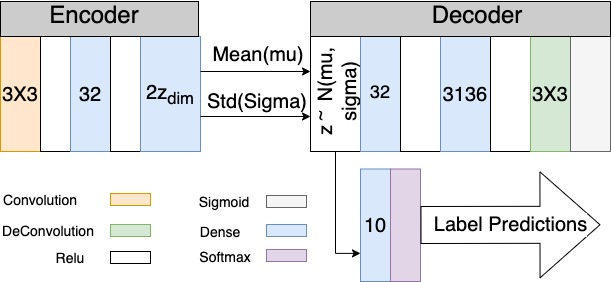
\includegraphics[width=2.1in]{images/var_arch_v5.jpg}
\DeclareGraphicsExtensions.
\caption{Proposed architecture. The VAE is augmented with a classification layer}
\label{vae_architecture}
\end{figure}
\section{Proposed Method}

\subsection{Dataset}
The proposed approach is demonstrated on the MNIST dataset.
The 50,000 training images are split into train (70\%) and validation (30\%) sets for hyper-parameter tuning.

\subsection{Neural Network Architecture}
Fig.\ref{vae_architecture} shows the architecture of the proposed model.
The model follows the usual encoder-decoder architecture of VAE.
The encoder consists of one down-sampling convolutional layer followed by two dense layers.
The decoder is made up of two dense layers and one up-sampling de-convolution layer.
An additional softmax classification layer was added to classify the latent vectors into one of the 10 class labels.

\subsection{Semi-supervised Loss Function and Training}\label{section_loss_function}
The VAE is initially trained until the reconstruction loss converges using the $\beta$-VAE loss function\cite{beta_vae} given below.
%\vspace{-0.3in}
\begin{equation} \label{vae_loss_eqn}
L_{VAE} = -\sum_{i, j}(x_{ij}^n \ln \hat{x}_{ij}^n
+ (1 - x_{ij}^n) \ln(1 -  \hat{x}_{ij}^n ) )\\
    +\beta KLD(p(z), N(0,I))
\end{equation}
where   $x_{ij}$ is the pixel value at position $(i, j)$ of the input image, $\hat{x}_{ij}$ is the pixel value of reconstructed image, $p(z)$ is the prior distribution of latent vectors, $N(0,I)$ is the standard multivariate normal distribution and KLD() denotes KL divergence.
Binary cross entropy loss is used as reconstruction loss for MNIST images, since the output activation function is sigmoid and MNIST images are treated as binary images in our experiments.

Once a reasonably good latent representation is learned using the loss function mentioned above, the latent vectors of the training samples are clustered into $k=10$ clusters.
The cluster centers were decoded and the resulting images were manually given a label and a confidence.
Fig.\ref{cluster_center_1} shows the reconstructed images of cluster centers after unsupervised training.

If the cluster center for a cluster does not correspond to any valid digit, all the samples in that cluster are again clustered into $k$ sub-clusters and  centers of the sub-clusters are labelled.
The process can be continued to form clusters at multiple levels based on the available manual annotation budget.
The labels assigned to the cluster center is then propagated to all other samples in the cluster using the following strategy:
\begin{enumerate}
    \item Each sample in the cluster is assigned with the  same label as the cluster center.
    \item Each sample is also given a confidence based on its distance from cluster center and  a manually assigned confidence in the range of [0,1]. The overall confidence of  training sample $x^n$ is computed as $w_n = p_cf(d_n)$
where $d_n$ is the distance of the sample from its cluster center, $p_c$  is the the cluster center confidence  and $f: d \mapsto [0,1]$ is a monotonically decreasing function that maps distance to a confidence value in unit interval [0,1].
\end{enumerate}

\begin{figure}
\centering
\begin{subfigure}[t]{.45\textwidth}
  \centering
  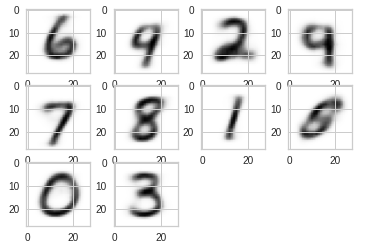
\includegraphics[width=.5\linewidth]{cluster_centers_epoch_1_0_gmm.png}
  \caption{With unsupervised training}
  \label{cluster_center_1}
\end{subfigure}\hfill
\begin{subfigure}[t]{.45\textwidth}
  \centering
  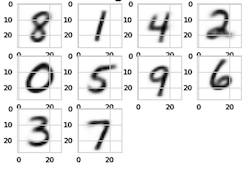
\includegraphics[width=.5\linewidth]{cluster_centers_epoch_5_0_gmm.png}
  \caption{Semi-supervised - 5 iterations}
  \label{cluster_center_5}
\end{subfigure}
\caption{Reconstructed images of cluster centers}
\label{cluster_center}
\end{figure}

Experiments were performed with different choices for  clustering algorithm (k-means and GMM), the distance metric (Euclidean and Mahalanobis) and confidence decay function- exponential (Equation \ref{exp_decay}) vs Gaussian (Equation \ref{gaussian_decay}).
\begin{equation}
    w_n = p_ce^{-a d_n}
    \label{exp_decay}
\end{equation}

\vspace{-0.2in}
\begin{equation}
    w_n = p_ce^{-a d_n^2}
    \label{gaussian_decay}
\end{equation}
where $a$ is a hyper parameter determining how fast the confidence decreases with the distance from cluster center.
With GMM, the product of posterior probability of the sample and cluster center confidence $p_c$ was used as the overall sample confidence.
Training is continued for more epochs using the modified loss function, given below, that incorporates the manual labels and confidence into account.
\begin{equation} \label{semi_supervised_loss}
L = L_{VAE}  - \gamma \sum_{k=0}^{K}w_{n}y_{nk}\ln(\hat{y}_{nk})
\end{equation}

where $y_{nk}$ is the one-hot encoded label and $\hat{y}_{nk}$ is the predicted softmax probability.
The new term added to the loss is the weighted multi-class cross entropy loss for classification task.

\section{Results and Discussions}

\begin{figure}
\centering
  \centering
  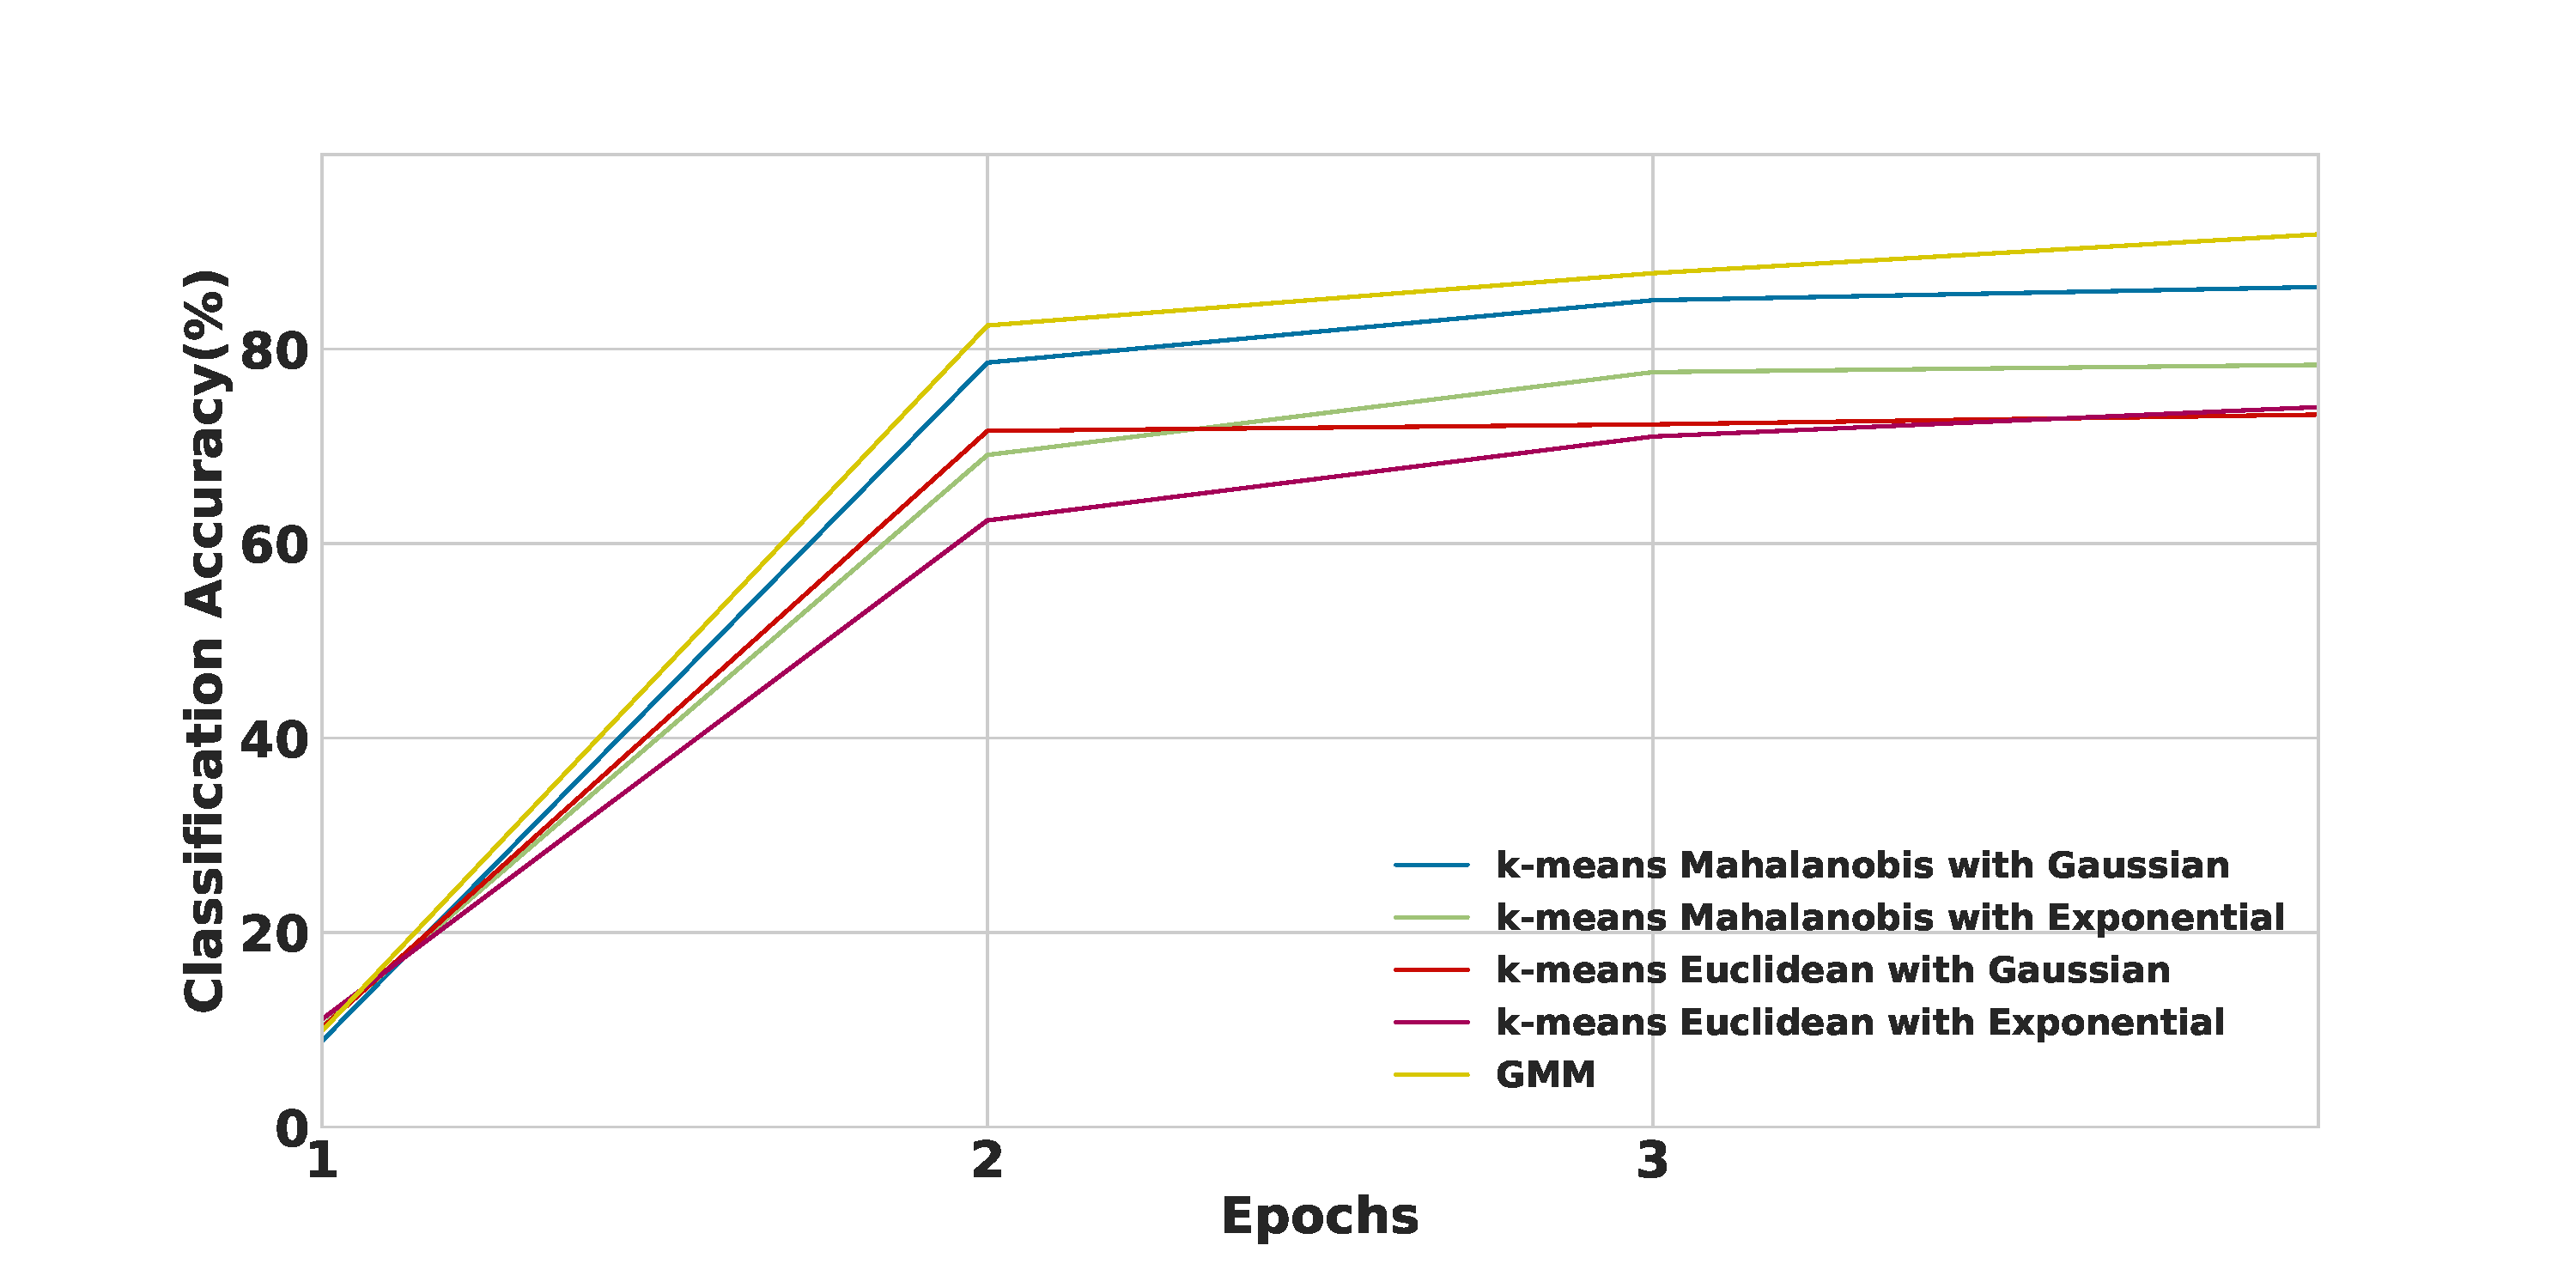
\includegraphics[width=.6\linewidth]{images/classification_accuracy_hyperparameter}
\caption{Comparison of classification accuracy with different choices of hyper-parameters distance metric, confidence function and clustering algorithms}
\label{classification_acc}
\end{figure}

In order to choose the optimum hyper-parameters like clustering algorithm, distance metric and confidence decay function, we ran experiments with different combinations of hyper parameters and the results are compared in Figures \ref{classification_acc}.
When k-means is used, performance is better with Gaussian confidence mapping function compared to exponential function.
This is expected as exponential function decreases at a faster rate near zero.
Hence, the confidence for samples closer to the cluster center decreases at a faster rate as it moves away from the cluster center.
Whereas  with Gaussian function, since the gradient of the curve is close to zero near cluster center, samples closer to the cluster center will have almost the same confidence as the cluster center confidence $p_c$.

With k-means clustering, using Mahalanobis distance instead of Euclidean distance gives a better classification accuracy.
Latent space distribution shown in Fig.\ref{tsne_semi_4_9} and Fig.\ref{tsne_semi}, shows that the clusters have different variance along different directions which is captured well in Mahalanobis distance.
For the same reason, GMM performs better than k-means clustering.

The reconstructed images of cluster centers shown in Fig.\ref{cluster_center} shows that as training progresses, the clusters formed in latent space correspond to different classes in MNIST dataset.
In Fig.\ref{cluster_center_1} some of the cluster centers do not correspond to any valid digit, and some digits like 4  are missing.
This is happening because the latent vectors for some classes, like  4 and 9 for example,  were very similar and got clustered into the same cluster.
However, after a few iterations of semi-supervised training, the latent vectors for symbol 9 and 4 are getting clustered into different clusters.
This is also evident from the t-SNE visualization of latent space shown in Fig.\ref{tsne_4_9}.

Fig.\ref{tsne} shows the 2-d t-SNE visualization of the latent vector distribution for the entire training set.
The distribution of samples from different classes becomes more separable with semi-supervised learning.
Fig.\ref{classificaion_acc} shows the  classification accuracy on test dataset.
Initial 10 epochs were trained in unsupervised mode and classification loss was added after that.
After 5 iterations of semi-supervised training, the classification accuracy increased to 93.9\% on MNIST test dataset.

\begin{figure}[!t]
\centering
  \centering
  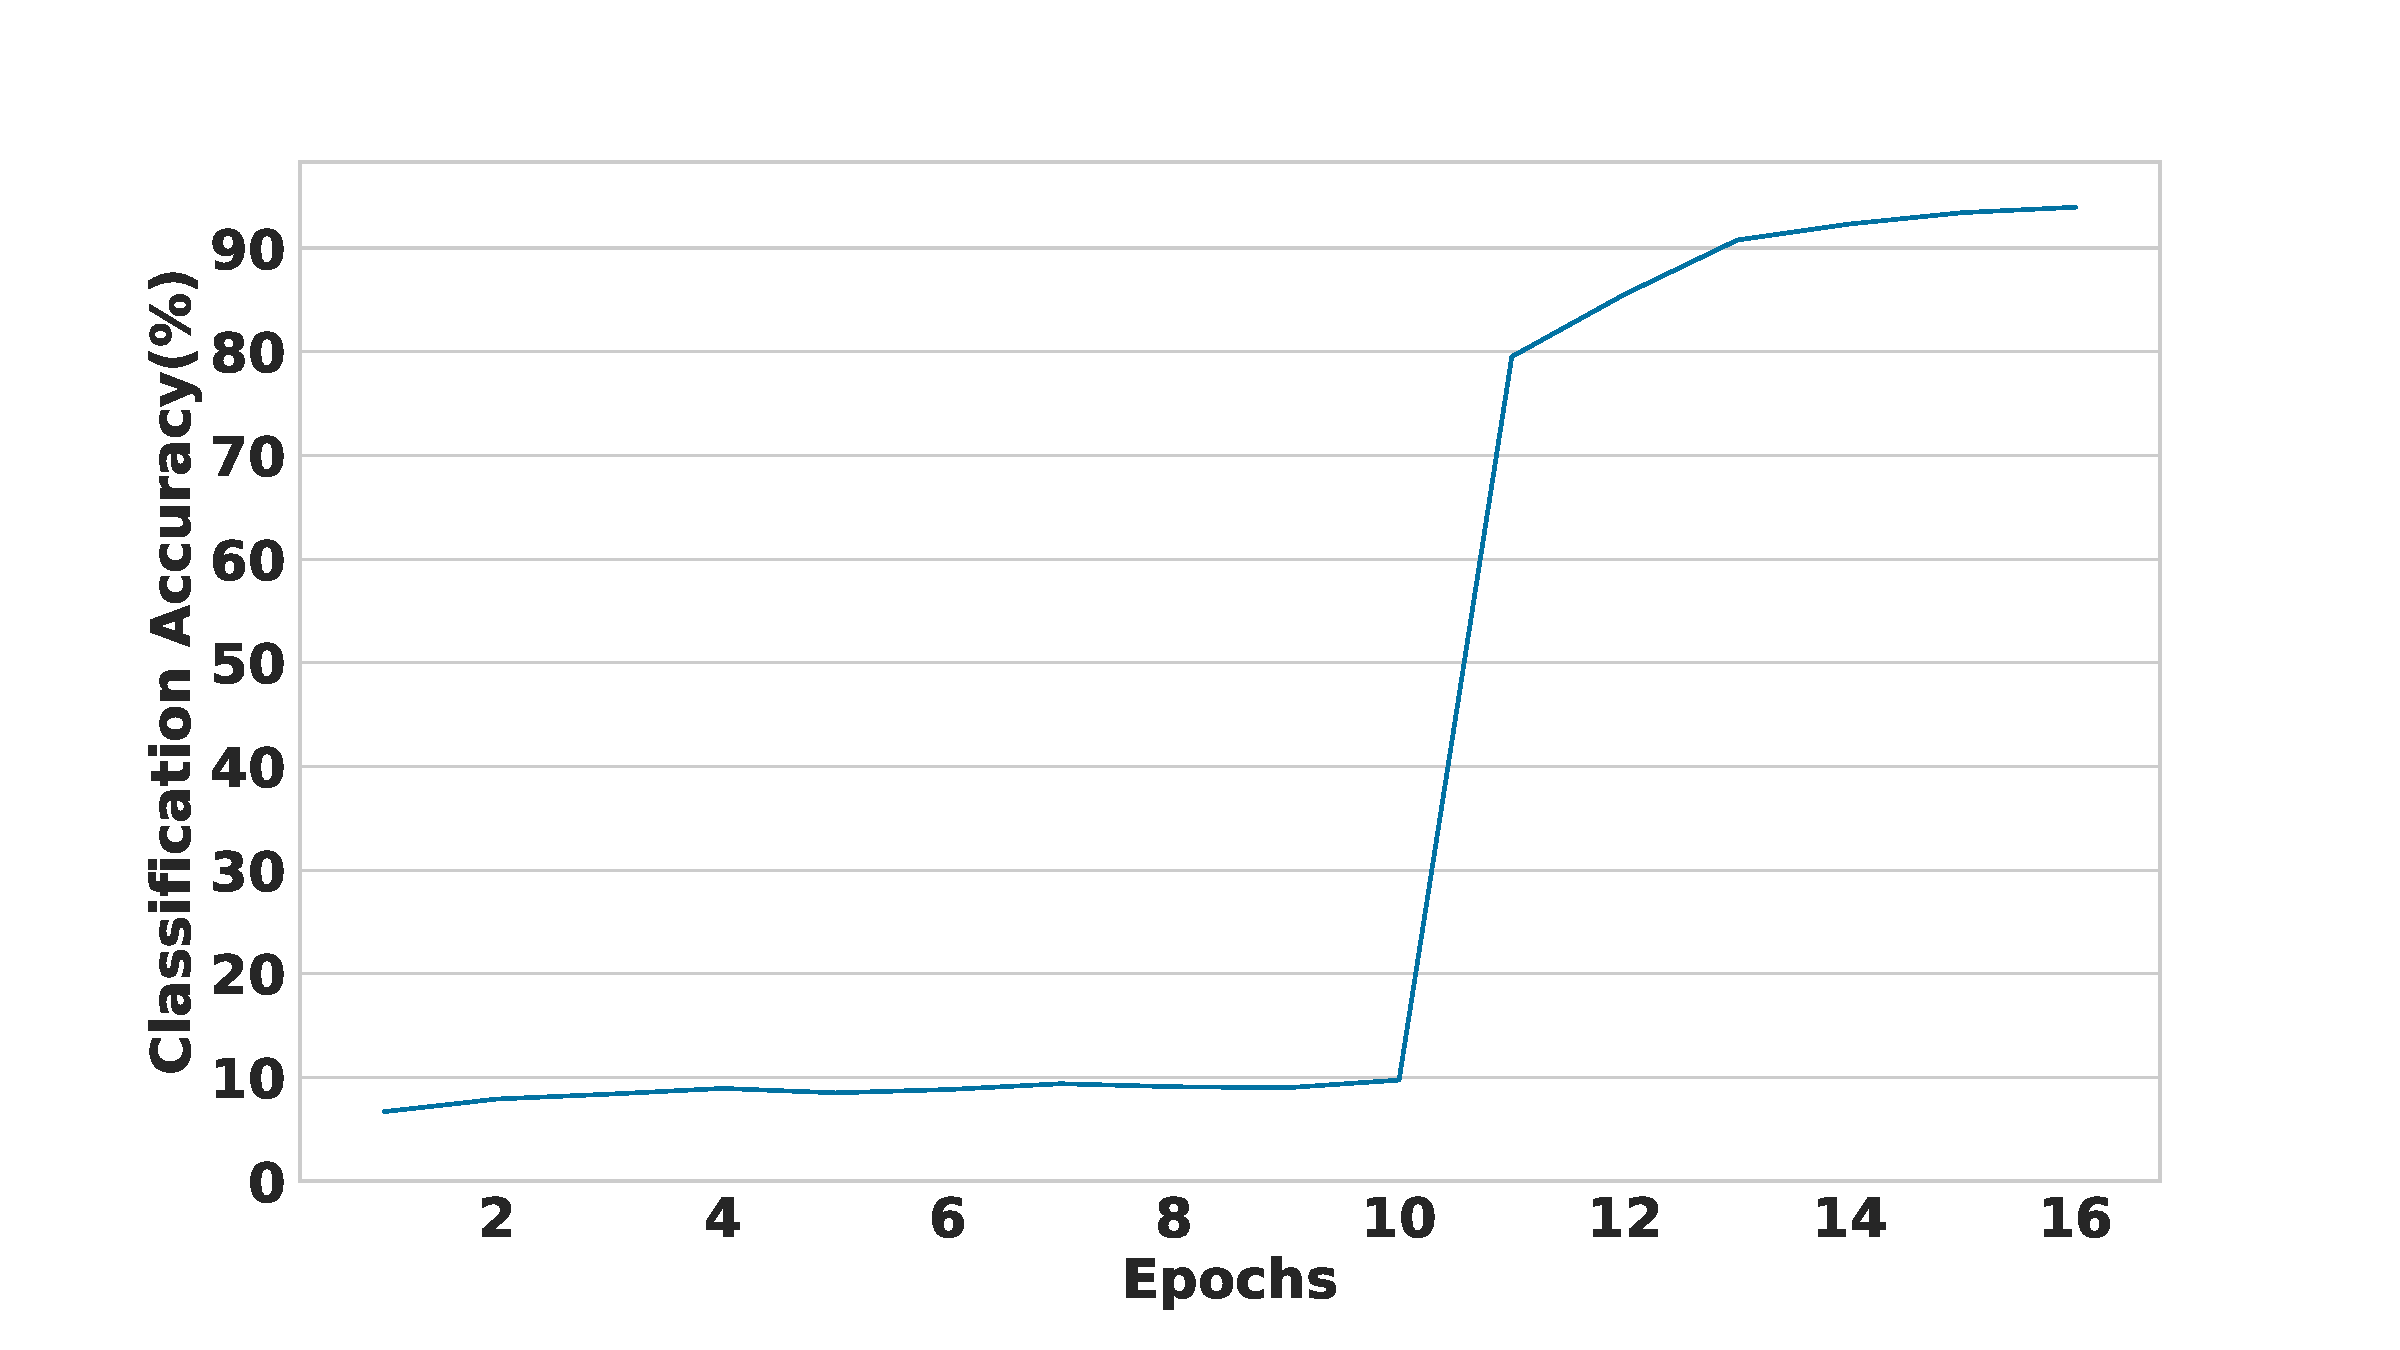
\includegraphics[width=.6\linewidth]{images/classification_acc_semi_supervised}
\caption{Classification accuracy on MNIST test dataset with 5 iterations of semi-supervised training. Classification loss was added after 10 epochs}
\label{classificaion_acc}
\end{figure}

\begin{figure}
\centering
\begin{subfigure}[t]{.4\textwidth}
  \centering
  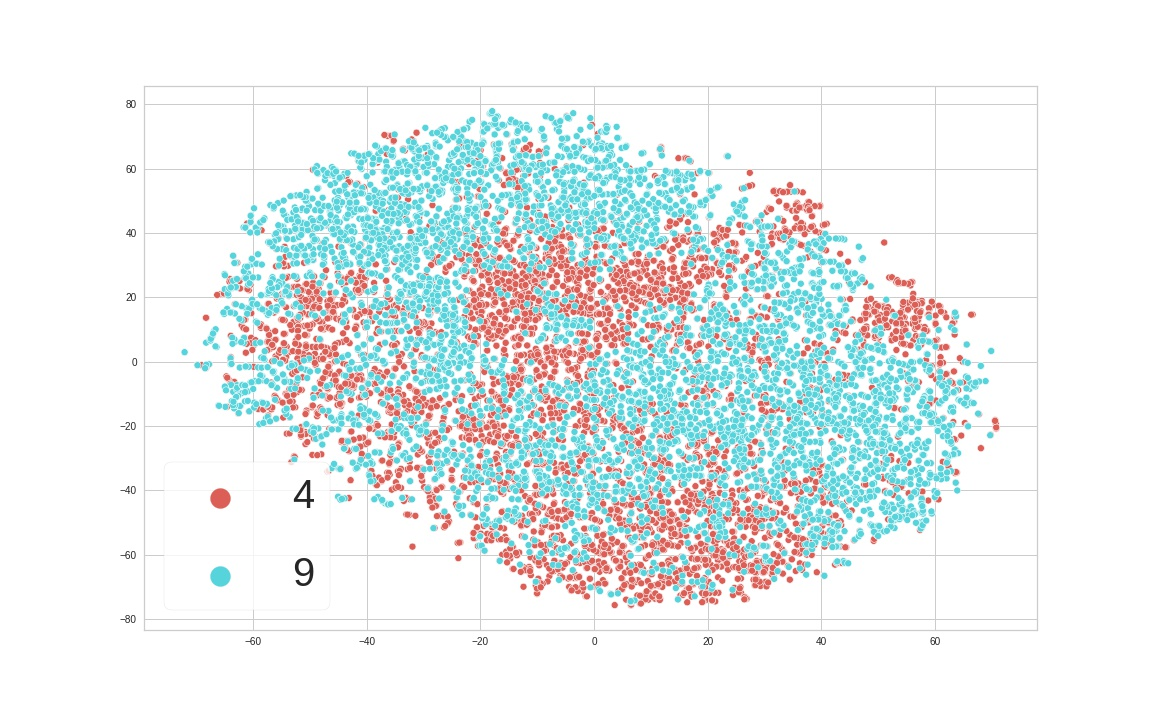
\includegraphics[width=0.8\linewidth]{images/tsne_4_9_unsup.jpg}
  \caption{Unsupervised training}
  \label{tsne_un_4_9}
\end{subfigure}\hfill
\begin{subfigure}[t]{.4\textwidth}
  \centering
  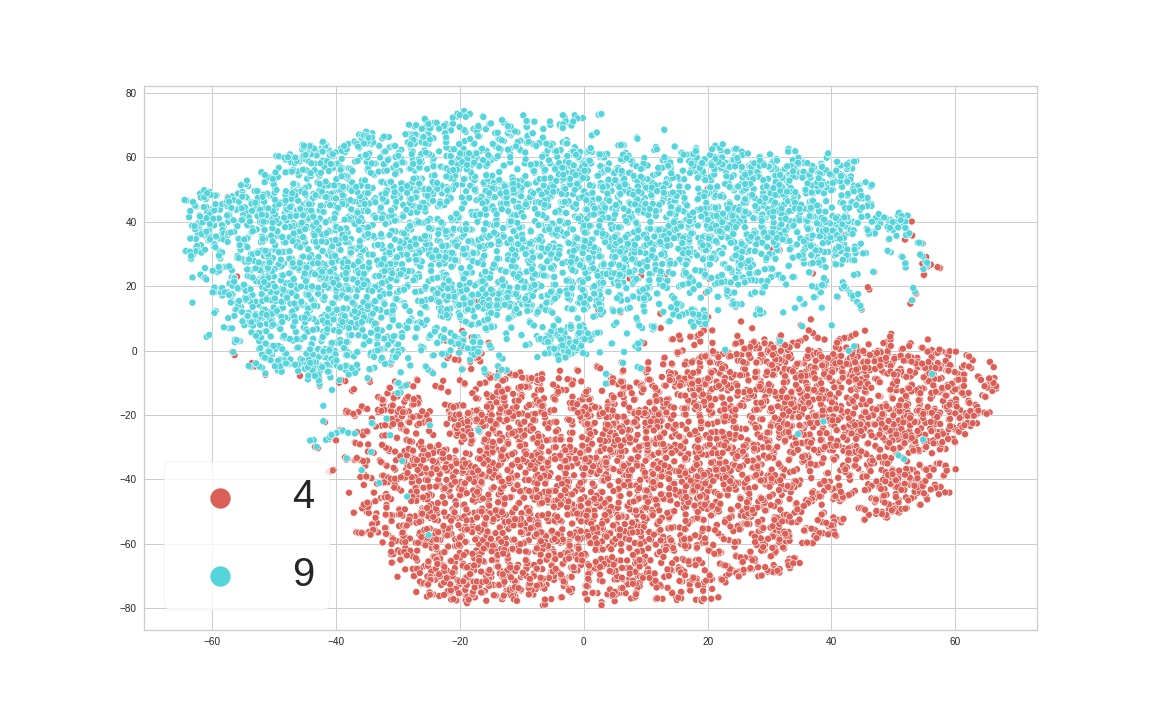
\includegraphics[width=0.8\linewidth]{images/tsne_4_9_semi.jpg}
  \caption{Semi-supervised - 5 iterations}
  \label{tsne_semi_4_9}
\end{subfigure}
\caption{Latent space distribution, with t-SNE, for samples from class 4 and 9}
\label{tsne_4_9}
\end{figure}

\begin{figure}[!h]
\centering
\begin{subfigure}[t]{.4\textwidth}
  \centering
  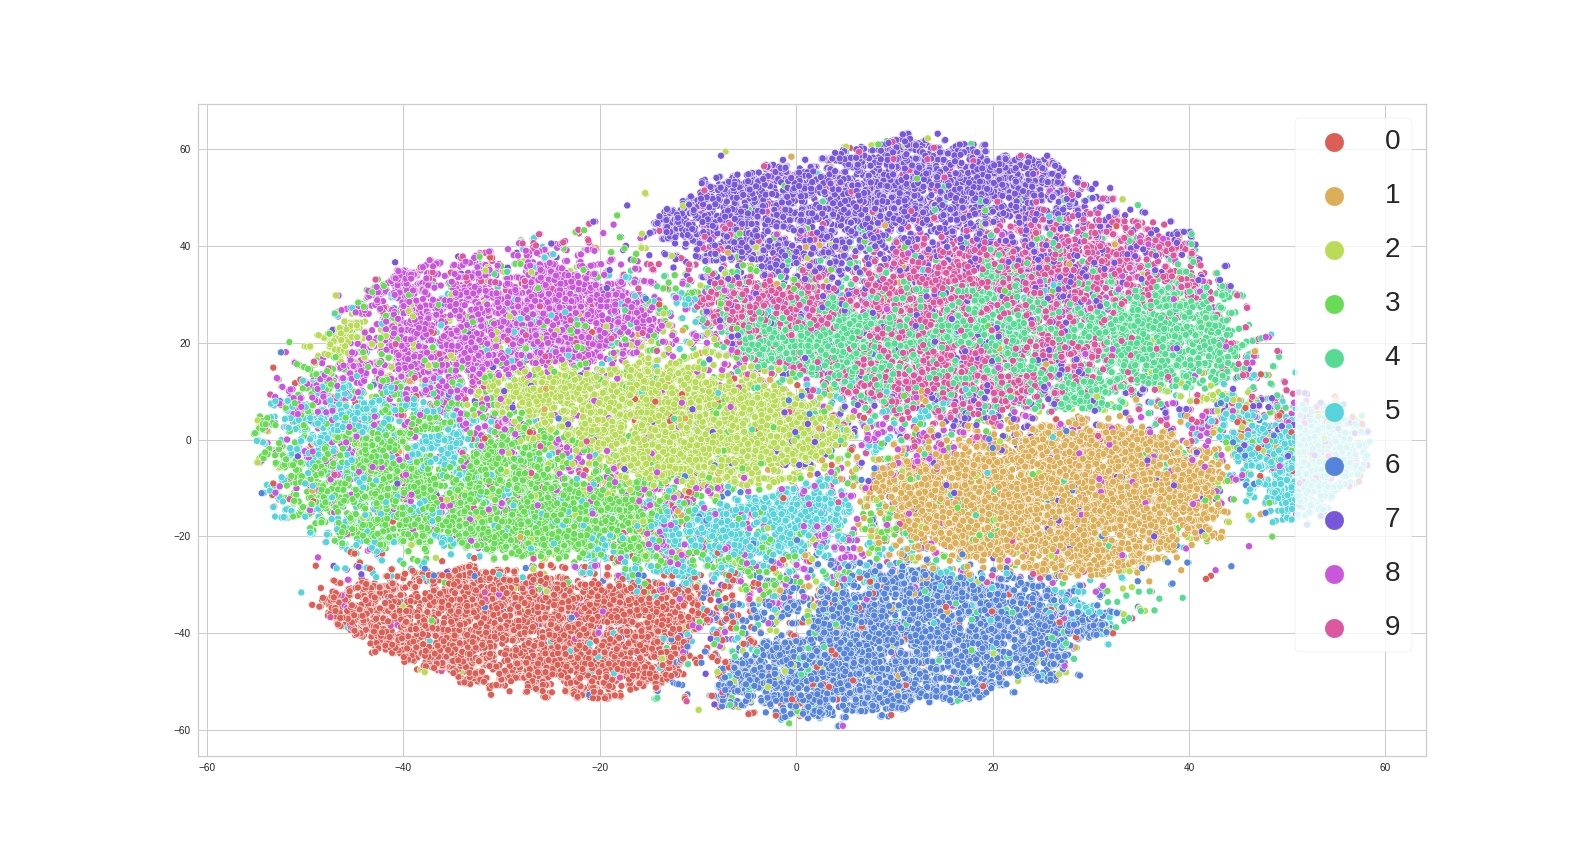
\includegraphics[width=.8\linewidth]{images/tsne_unsup.jpg}
  \caption{Unsupervised training}
  \label{tsne_un}
\end{subfigure}\hfill
\begin{subfigure}[t]{.4\textwidth}
  \centering
  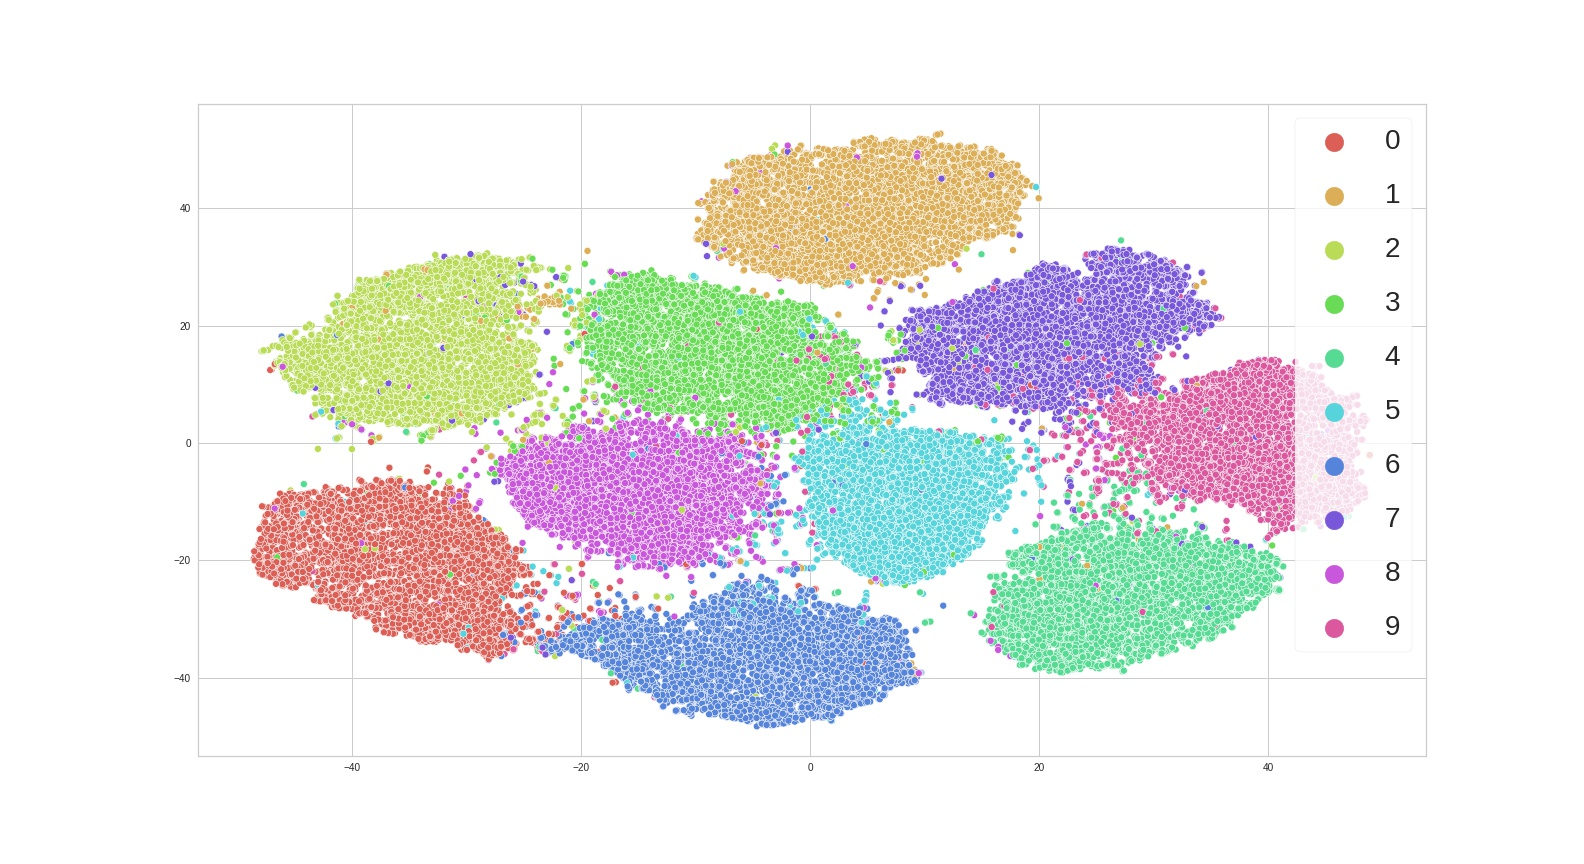
\includegraphics[width=.8\linewidth]{images/tsne_semi.jpg}
  \caption{Semi-supervised - 5 iterations }
  \label{tsne_semi}
\end{subfigure}
\caption{Latent space distribution for the entire training set. With semi-supervised training, semantically valid and well separated clusters are formed}
\label{tsne}
\end{figure}
\section{Conclusion}
In this paper, we propose a novel deep learning based active learning framework for solving complex tasks like image classification using clusters formed in the low dimensional latent space learned by a variational autoencoder.
Our approach is demonstrated by classifying MNIST images without using labels provided in the dataset.
We performed multiple experiments with different choices for hyper parameters like clustering algorithm, distance metric and confidence function.
Our experiments show that GMM, when used as a clustering algorithm,  gives the best classification accuracy of 93.9\% on the MNIST test dataset after 5 iterations.
It is observed, using 2-d t-SNE visualization, that  semantically valid and separable clusters are formed as a result of semi-supervised learning.


% \clearpage
%
% ---- Bibliography ----
%
% BibTeX users should specify bibliography style 'splncs04'.
% References will then be sorted and formatted in the correct style.
%
\bibliographystyle{splncs04}
%\bibliography{semisupervised.bib}
%
\begin{thebibliography}{8}
    \bibitem{alexnet}
    Krizhevsky, Alex, Ilya Sutskever, and Geoffrey E. Hinton. Imagenet classification with deep convolutional neural networks. Advances in neural information processing systems 25 (2012): 1097-1105
    \bibitem{vggnet}
    Simonyan, Karen, and Andrew Zisserman. Very deep convolutional networks for large-scale image recognition. 3rd International Conference on Learning Representations, {ICLR} 2015.
    \bibitem{resnet}
    He, Kaiming, et al. Deep residual learning for image recognition. Proceedings of the IEEE conference on computer vision and pattern recognition. 2016.
    \bibitem{deeplab}
    Chen, Liang-Chieh, et al. Deeplab: Semantic image segmentation with deep convolutional nets, atrous convolution, and fully connected crfs. IEEE transactions on pattern analysis and machine intelligence 40.4 (2017): 834-848.
    \bibitem{unet}
    Ronneberger, Olaf, Philipp Fischer, and Thomas Brox. U-net: Convolutional networks for biomedical image segmentation. International Conference on Medical image computing and computer-assisted intervention. Springer, Cham, 2015.
    \bibitem{yolo}
    Redmon, Joseph, et al. You only look once: Unified, real-time object detection. Proceedings of the IEEE conference on computer vision and pattern recognition. 2016.
    \bibitem{faster_rcnn}
    Ren, Shaoqing, et al. Faster r-cnn: Towards real-time object detection with region proposal networks. Advances in neural information processing systems 28 (2015): 91-99.
    \bibitem{beta_vae}
    Higgins, Irina, et al. beta-vae: Learning basic visual concepts with a constrained variational framework. (2016)
    \bibitem{kingma_2014}
    Kingma, Diederik P., et al. Semi-supervised learning with deep generative models. Advances in Neural Information Processing Systems 2014.
    \bibitem{vaal}
    Sinha, Samarth, Sayna Ebrahimi, and Trevor Darrell. Variational adversarial active learning. Proceedings of the IEEE/CVF International Conference on Computer Vision. 2019
    \bibitem{vae}
    Kingma, Diederik P., and Max Welling. Auto-encoding variational bayes. 2nd International Conference on Learning Representations, {ICLR} 2014.
    \bibitem{gan}
    Goodfellow, Ian, et al. Generative adversarial nets. Advances in neural information processing systems 27 (2014).
    \bibitem{mahapatra_2018}
    Mahapatra, Dwarikanath, et al. Efficient active learning for image classification and segmentation using a sample selection and conditional generative adversarial network. International Conference on Medical Image Computing and Computer-Assisted Intervention. Springer, Cham, 2018.
    \bibitem{mayer_2020}
    Mayer, Christoph, and Radu Timofte. Adversarial sampling for active learning. Proceedings of the IEEE/CVF Winter Conference on Applications of Computer Vision. 2020.
    \bibitem{wang_2016}
    Wang, Keze, et al. Cost-effective active learning for deep image classification. IEEE Transactions on Circuits and Systems for Video Technology 27.12 (2016): 2591-2600.
    \bibitem{beluch_2018}
    Beluch, William H., et al. The power of ensembles for active learning in image classification. Proceedings of the IEEE Conference on Computer Vision and Pattern Recognition. 2018.
    \bibitem{mikhail_2006}
    Belkin, Mikhail, Partha Niyogi, and Vikas Sindhwani. Manifold regularization: A geometric framework for learning from labeled and unlabeled examples. Journal of machine learning research 7.11 (2006).
    \bibitem{ding_2018}
    Ding, S., Xi, X., Liu, Z. et al. A Novel Manifold Regularized Online Semi-supervised Learning Model. Cogn Comput 10, 49–61 (2018).
    \bibitem{li_2018}
    Li, Qimai, Zhichao Han, and Xiao-Ming Wu. Deeper insights into graph convolutional networks for semi-supervised learning. Thirty-Second AAAI conference on artificial intelligence. 2018.
    \bibitem{joachims_1999}
    Joachims, Thorsten. Transductive inference for text classification using support vector machines. Icml. Vol. 99. 1999.
    \bibitem{bennett_1999}
    Bennett, Kristin, and Ayhan Demiriz. Semi-supervised support vector machines. Advances in Neural Information processing systems (1999): 368-374.
\end{thebibliography}
\end{document}
